\section{Large Scale Image Reconstruction for the MeerKAT Telescope} \label{intro}
Image reconstruction

Applying the theory of compressed sensing to certain reconstruction problems, because they are we have theoretical guarantees with them.

Compressed Sensing reconstructions useful for incomplete measurements

Applied to the radio interferometer MeerKAT, which has the following measurement equation \eqref{intro:measurement}.
\begin{equation}\label{intro:measurement}
V(u, v) = \int\int X(x, y) e^{2 \pi i (ux+vy)} \: dx \: dy 
\end{equation}

Radio interferometers observe the image $X$, but they do not measure pixel locations, they measure Fourier Components $V$ of the sky at continuous locations $u, v$. The image reconstruction wants to find the observed image $X$ from the measured Visibilities $V$. Calculating the image would be calculating the two dimensional inverse Fourier Transform of $V$, but two properties make the problem harder:

\begin{enumerate}
	\item Non-uniform sampling pattern in Visibility space
	\item Incomplete Visibilities
\end{enumerate}

We are interested in an image $X$ with uniformly sized pixels. The instrument measures areas in Visibility space more densely than others. This property keeps us away from the Fast Fourier Transform. The inverse Fourier Transform can still be calculated, but it results in an algorithm with quadratic runtime. It is not practical.

Incomplete measurements create wrong artefacts in the image. Reconstructing the image is finding out which structures are plausible and which are not.

Reconstructing the image $X$ requires therefore solving two problems:
\begin{enumerate}
	\item Creating a fast image with uniform pixels from non-uniform Visibilities.
	\item Deciding which image structures are plausible.
\end{enumerate}

Current algorithms solve these two problems all the same way. They use the major cycle architecture.


\subsection{The Major Cycle Architecture}
The major cycle architecture was conceived for the CLEAN class of algorithm. Compressed sensing approaches use essentially the same architecture. The figure \ref{intro:major} shows the major cycle framework. In a major cycle consists of two parts: The non-uniform FFT and an optimization algorithm.

Together, they form the major cycle which solves the two problems over several iterations. 

\begin{wrapfigure}{r}{0.6\textwidth}
	\centering
	\vspace{-10pt}
	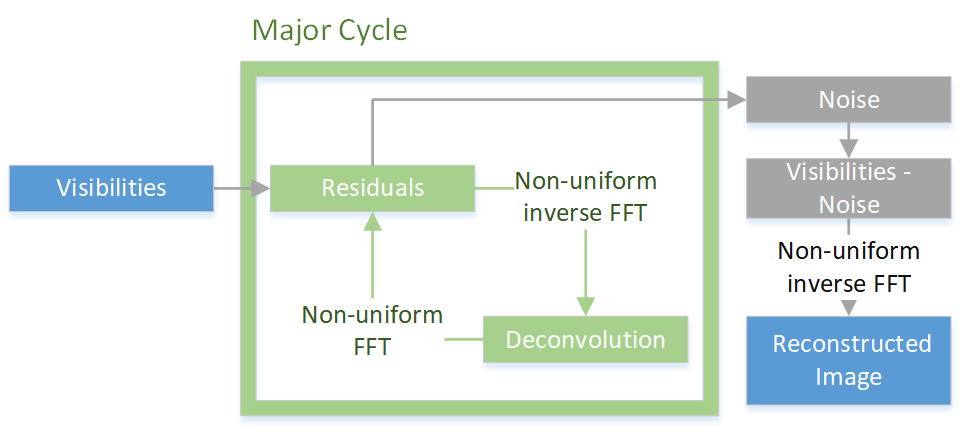
\includegraphics[width=1.0\linewidth]{./chapters/01.intro/Major-Minor.png}
	\caption{The Major Cycle Framework}
	\label{intro:major}
	\vspace{-10pt}
\end{wrapfigure}

The non-uniform FFT is responsible for approximating a regularly spaced image from the measurements, and for approximating the measurements corresponding to an image. Non-uniform FFT's are fast approximation algorithms, but by being approximation algorithms, they introduce errors. 

A optimization algorithm uses the image and removes the effect of incomplete samples. In the past, CLEAN algorithms were used to remove the effects. For the future, algorithms based on the theory of compressed sensing show promises in image quality.

A full major cycle consists of the following operations: First, it approximates the regularly spaced the regularly spaced image from the measurements. Then the optimization algorithm removes the effects of Incomplete measurements and returns the corresponding image. The major cycle then approximates the measurements corresponding to the image with the non-uniform FFT. The residual measurements are used in the next Major Cycle. In each cycle, two errors get simultaneously reduced:

\begin{enumerate}
	\item The Error introduced by the non-uniform FFT.
	\item The Error introduced by the incomplete measurements.
\end{enumerate}

After several major cycles the algorithm converges on a regularly spaced image which has a small error from non-uniform samples, and a small error from incomplete measurements.

For the optimization algorithm, the CLEAN class of algorithms get used. But algorithms based on the theory of compressed sensing have been shown to produce superior images.


\subsection{Compressed Sensing Reconstructions}
 However, compressed Sensing algorithms come with the drawback of requiring more major cycles.

Current Compressed Sensing reconstructions reduce the number of major cycles. However, the question is if Compressed Sensing can use a different architecture, and scale better to problems of the size of MeerKAT.

Furthermore on the new MeerKAT instruments, we have a big data problem. We want to create a large image from a large amount of Visibilities. 32k*32k pixels and terabytes of raw Visibility data. 

Scalability is a big problem.

There are ways to get rid of the major cycle, but overall the complexity could not be reduced.









